\chapter{线性代数}

\marginpar{
  \begin{center}
    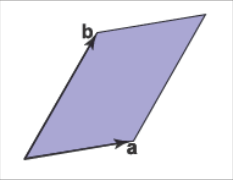
\includegraphics[width=0.25\textwidth]{6.1.png}
    \captionof{figure}{这个平行四边形的带符号面积是 $|ab|$ ,并且在这种情况下面积为正。}
  \end{center}
}

\marginpar{
  \begin{center}
    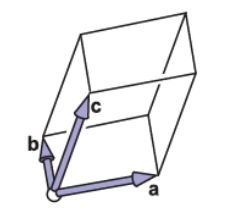
\includegraphics[width=0.25\textwidth]{6.2.png}
    \captionof{figure}{所示平行六面体的带符号体积由行列式$|abc|$表示,在这种情况下,体积为正,因为这个向量以右旋作为基准。}
  \end{center}
}

\marginpar{
  \begin{center}
    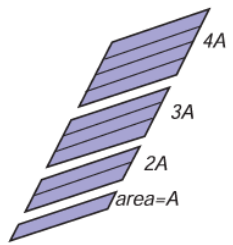
\includegraphics[width=0.25\textwidth]{6.3.png}
    \captionof{figure}{沿一个方向缩放平行四边形会以相同比例改变面积。}
  \end{center}
}

图形程序中最通用的工具恐怕就是改变或转换点和向量的矩阵了。在接下来的章节中,我们将学习如何将一个向量表示为一个只有一列的矩阵,并且通过矩阵乘法用不同的方式表示该向量。我们还将描述如何使用这种乘法来完成对向量的改变,比如缩放、旋转和平移。在这一章中,我们从几何学的角来回顾线性代数基础,专注于直感和在二维、三维上行之有效的算法。

对自己线性代数知识掌握有信心的读者可跳过这个章节,尽管如此,这里还是有些小道消息可能会对你有所启发,例如行列式的发展以及对奇异值和特征值分解的讨论等。

\section{行列式}

\marginpar{
  \begin{center}
    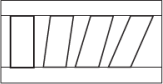
\includegraphics[width=0.25\textwidth]{6.4.png}
    \captionof{figure}{剪切平行四边形不会改变其面积。这四个平行四边形底相同,因此面积也相同。}
  \end{center}
}

\marginpar{
  \begin{center}
    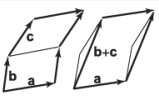
\includegraphics[width=0.25\textwidth]{6.5.png}
    \captionof{figure}{方程式6.1后面的几何结构。左边两个平行四边形可以被剪切成右边的平行四边形。}
  \end{center}
}

我们通常认为行列式是在线性方程的解中出现的。然而,在此处,我们有意将行列式视为另一种向量相乘的方式。对于二维向量$a$和$b$,行列式$|ab|$是$a$和$b$形成的平行四边形的面积(图6.1)。这是一个带符号的面积,并且当$a$和$b$右旋时符号为正,左旋则为负,也就是$|ab| = -|ba|$。在二维中,我们可以把“右旋”理解为逆时针旋转第一个向量至与第二个向量形成最小的角。三维中的行列式则必须同时计算三个向量。对于三个三维向量$a$、$b$和$c$,行列式$|abc|$是这三个向量形成的平行六面体(三维平行四边形;一个修剪的三维盒子)的带符号体积(图6.2)。

要计算一个二维行列式,首先需要确定它的一些性质。我们注意到对平行四边形的其中一条边进行缩放,与它面积缩放的比例是相同的(图6.3):
\[
  |(ka)b| =  |a(kb)| = k|ab|
\]
此外,“修剪”一个平行四边形不会改变它的面积(图6.4):
\[
  |(a+kb)b| =  |a(b+ka)| = |ab|
\]
最终我们发现,行列式拥有如下特性:
\begin{equation}
  |a(b+c)| =  |ab| + |ac|
\end{equation}
如图6.5所示,我们可以滑动两个平行四边形中间的边来形成一个平行四边形而不改变原来两个平行四边形的面积。

现在让我们假设a和b的笛卡尔表示法:
\[
  \begin{aligned}
    |ab| & = |(x_aX + y_aY)(x_bX + y_bY)| \nonumber               \\
         & =x_ax_b|XX|+x_ay_b|XY|+y_ax_b|YX|+y_ay_b|YY| \nonumber \\
         & =x_ax_b(0)+x_ay_b(+1)+y_ax_b(-1)+y_ay_b(0) \nonumber   \\
         & = x_a y_b - y_a x_b \nonumber
  \end{aligned}
\]
简而言之,对于任何向量v,都有|vv|=0,即平行四边形四边共线,因此没有面积。

在三维空间中,三个三维向量$a$、$b$和$c$的行列式记作$|abc|$。这些向量的笛卡尔表示对于平行六面体和平行四边形具有相似的规则,并且我们可以像对二维那样进行类似的拓展:
\begin{equation}
  \begin{aligned}
    |abc| & = |(x_aX+y_aY+z_aZ)(x_bX+y_by+z_bZ)(x_cX+y_cY+z_cZ)| \nonumber          \\
          & =x_ay_bz_c-x_az_by_c-y_ax_bz_c+y_az_bx_c+z_ax_by_c-z_ay_bx_c \nonumber.
  \end{aligned}
\end{equation}
可以看到,这种方式下行列式的计算随着维度的升高变得越来越糟糕。我们将在章节6.3.2讨论易错更少的计算方法。

\textcolor{purple}{例二:}

\begin{figure}[htbp]
  \centering
  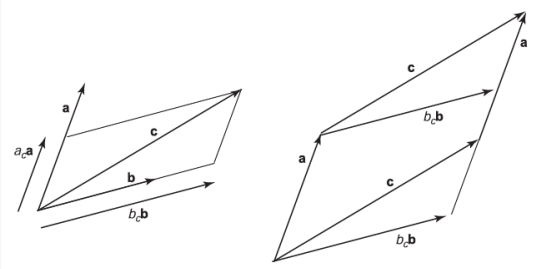
\includegraphics[width=1.0\textwidth]{6.6.png}
  \caption{左侧的向量c可以用两个基向量表示成$a_ca+b_cb$。我们看到右侧,由$a$和$c$形成的平行四边形是由$b_b$和$a$形成的平行四边形的剪切版本。}
\end{figure}

行列式自然产生于计算一个向量的表达式作为其他两个的线性组合——举个例子,如果我们希望用向量$c$表示一个向量组合$a$和$b$:
\[
  c = a_a + b_cb
\]
参照图6.6得到:
\[
  |(b_cb)a| = |ca|
\]
因为这些平行四边形只是彼此的剪切版本。解出$b_c$为
\[
  b_c = |ca|/|ba|
\]
类比得出
\[
  a_c = |bc|/|ba|
\]
这是克莱姆法则的二维版本,我们将在章节6.3.2中再次探讨。

\section{矩阵}

矩阵是一个遵循某些算术规则的数值元素的数组。这是一个两行三列的矩阵示例:
\[
  \left[\begin{array}{rrr}
      1.7 & -1.2 & 4.2  \\
      3.0 & 4.5  & -7.2
    \end{array}\right]
\]
计算机图形学频繁地用到矩阵解决各种问题,例如空间变换的表示。在我们的讨论中,假设矩阵的元素都是实数。这个章节描述矩阵算法的力学原理和“方形”矩阵(译者注:即方阵,行数和列数相同的矩阵)的行列式。

\subsection{\textcolor{lightgreen}{矩阵计算}}

矩阵乘以一个常数会得到一个矩阵,其中每个元素都会乘以这个常数,例如:
\[
  2\left[\begin{array}{rr}
      1 & -4 \\
      3 & 2
    \end{array}\right]=\left[\begin{array}{rr}
      2 & -8 \\
      6 & 4
    \end{array}\right]
\]
矩阵还可以逐个元素对应相加,例如:
\[
  \left[\begin{array}{rr}
      1 & -4 \\
      3 & 2
    \end{array}\right]+\left[\begin{array}{ll}
      2 & 2 \\
      2 & 2
    \end{array}\right]=\left[\begin{array}{rr}
      3 & -2 \\
      5 & 4
    \end{array}\right]
\]
对于矩阵乘法,我们将第一个矩阵的行与第二个矩阵的列“相乘”:
\[
  \begin{bmatrix}
    a_{11} & \cdots & a_{1m} \\
    \vdots &        & \vdots \\
    a_{i1} & \cdots & a_{im} \\
    \vdots &        & \vdots \\
    a_{r1} & \cdots & a_{rm}
  \end{bmatrix}
  \begin{bmatrix}
    b_{11} & \cdots & b_{1j} & \cdots & b_{1c} \\
    \vdots &        & \vdots &        & \vdots \\
    b_{m1} & \cdots & b_{mj} & \cdots & b_{mc} \\
  \end{bmatrix}
  =
  \begin{bmatrix}
    p_{11} & \cdots & p_{1j} & \cdots & p_{1c} \\
    \vdots &        & \vdots &        & \vdots \\
    p_{i1} & \cdots & p_{ij} & \cdots & p_{ic} \\
    \vdots &        & \vdots &        & \vdots \\
    p_{r1} & \cdots & p_{rj} & \cdots & p_{rc}
  \end{bmatrix}
\]
因此元素$p_{ij}$的乘积结果是:
\begin{equation}
  p_{ij} = a_{i1}b_{1j} + a_{i2}b_{2j}+ \cdots + a_{im}b_{mj}
\end{equation}
只有当左边矩阵的列数与右边矩阵的行数相同时,才能取得两个矩阵的乘积。例如:
\[:\left[\begin{array}{ll}
      0 & 1 \\
      2 & 3 \\
      4 & 5
    \end{array}\right]\left[\begin{array}{llll}
      6 & 7 & 8 & 9 \\
      0 & 1 & 2 & 3
    \end{array}\right]=\left[\begin{array}{rrrr}
      0  & 1  & 2  & 3  \\
      12 & 17 & 22 & 27 \\
      24 & 33 & 42 & 51
    \end{array}\right]
\]
矩阵乘法在大多数情况下都不满足交换律:
\begin{equation}
  \mathbf{AB} \neq \mathbf{BA}
\end{equation}
同样,如果$\mathbf{AB} = \mathbf{AC}$,它并不一定满足$\mathbf{B} = \mathbf{C}$。幸运的是,矩阵乘法满足结合律和分配律:
\[
  \begin{aligned}
    (\mathbf{A B}) \mathbf{C}          & =\mathbf{A}(\mathbf{B C})  \\
    \mathbf{A}(\mathbf{B}+\mathbf{C})  & =\mathbf{A B}+\mathbf{A C} \\
    (\mathbf{A}+\mathbf{B}) \mathbf{C} & =\mathbf{A C}+\mathbf{B C}
  \end{aligned}
\]

\subsection{\textcolor{lightgreen}{矩阵运算}}

我们想得到一个逆矩阵。首先我们知道实数$x$的倒数是$1/x$,并且他们的乘积为1。我们需要一个矩阵$\mathbf{I}$看作是一个“矩阵1”。它只存在于方阵中,并称之为\textit{单位方阵};它由\textit{主对角线}的1和其它地方的0组成。例如,4×4的单位阵是:
\[
  \mathbf{I}=\left[\begin{array}{llll}
      1 & 0 & 0 & 0 \\
      0 & 1 & 0 & 0 \\
      0 & 0 & 1 & 0 \\
      0 & 0 & 0 & 1
    \end{array}\right]
\]

矩阵$\mathbf{A}$的逆矩阵$\mathbf{A}^{-1}$是使得$\mathbf{A}\mathbf{A}^{-1} = \mathbf{I}$的矩阵。例如:
\[
  \left[\begin{array}{ll}
      1 & 2 \\
      3 & 4
    \end{array}\right]^{-1}=\left[\begin{array}{rr}
      -2.0 & 1.0  \\
      1.5  & -0.5
    \end{array}\right] \text { 因为 }\left[\begin{array}{ll}
      1 & 2 \\
      3 & 4
    \end{array}\right]\left[\begin{array}{rr}
      -2.0 & 1.0  \\
      1.5  & -0.5
    \end{array}\right]=\left[\begin{array}{ll}
      1 & 0 \\
      0 & 1
    \end{array}\right]
\]
$\mathbf{A}^{-1}$的逆记作$\mathbf{A}$,因此$\mathbf{AA}^{-1} = \mathbf{A}^{-1}\mathbf{A} = \mathbf{I}$。
两个矩阵乘积的逆是两个矩阵逆的乘积,但顺序交换。
\begin{equation}
  (\mathbf{A B})^{-1} = \mathbf{B}^{-1} \mathbf{A}^{-1}
\end{equation}
章节6.3我们将回到这个计算逆的问题。

矩阵$\mathbf{A}$的\it{转置}$\mathbf{A^T}$拥有与之相同的数字,但行和列被交换了。如果我们把$\mathbf{A^T}$的条目记作$\mathbf{a'_{ij}}$,则:
\[
a_{ij} = a'_{ji}
\]
例如:
\[
  \left[\begin{array}{ll}
      1 & 2 \\
      3 & 4 \\
      5 & 6
    \end{array}\right]^{\mathrm{T}}=\left[\begin{array}{lll}
      1 & 3 & 5 \\
      2 & 4 & 6
    \end{array}\right]
\]
两个矩阵乘积的转置遵循于方程6.4相似的规则:\[(\mathbf{AB})^T=\mathbf{B}^T\mathbf{A}^T\]

方阵的行列式就是这个矩阵列的行列式,被认为是一组向量。这个行列式与刚才讨论的矩阵运算有几个不错的关联,在这里列出以供参考:
\begin{align}
  |\mathbf{A B}|                       & = |\mathbf{A}| |\mathbf{B}| \\
  \left|\mathbf{A}^{-1}\right|         & = \frac{1}{|\mathbf{A}|}    \\
  \left|\mathbf{A}^{\mathrm{T}}\right| & = |\mathbf{A}|
\end{align}

\subsection{\textcolor{lightgreen}{矩阵形式的向量运算}}

在图形中,我们使用一个方阵来变换一个表示为矩阵的向量。比如有一个二维向量$a = (x_a,y_a)$要绕原点旋转90度得到向量$a' = (-y_a,x_a)$,可以用一个2×2的矩阵和一个2×1的矩阵来计算乘积,称为\it{列向量}。这个计算的矩阵形式是:
\[
  \left[\begin{array}{rr}
      0 & -1 \\
      1 & 0
    \end{array}\right]\left[\begin{array}{l}
      x_{a} \\
      y_{a}
    \end{array}\right]=\left[\begin{array}{r}
      -y_{a} \\
      x_{a}
    \end{array}\right]
\]
我们也可以通过这个矩阵的转置左乘(“前相乘”)一个行向量得到相同的结果:
\[
  \left[\begin{array}{ll}
      x_{a} & y_{a}
    \end{array}\right]\left[\begin{array}{rr}
      0  & 1 \\
      -1 & 0
    \end{array}\right]=\left[\begin{array}{ll}
      -y_{a} & x_{a}
    \end{array}\right]
\]
现如今,使用列向量的后乘法是绝对标准的,但在很多早期的书籍和系统中,会看到行向量和前乘法。

我们也可以用矩阵形式来编码仅对向量的操作。如果我们把点积的结果看作是一个1×1的矩阵,可以写作:\[a·b = a^Tb\]例如,如果我们取两个三维向量,会得到:
\[
  \left[\begin{array}{lll}
      x_{a} & y_{a} & z_{a}
    \end{array}\right]\left[\begin{array}{l}
      x_{b} \\
      y_{b} \\
      z_{b}
    \end{array}\right]=\left[x_{a} x_{b}+y_{a} y_{b}+z_{a} z_{b}\right]
\]

一组相关的向量乘积是两个向量的\text{外积},可以表示成左侧是列向量,右侧是行向量的矩阵乘法:$\mathbf{ab}^T$。结果是一个由$a$和$b$中所有条目对应的乘积构成的矩阵。对于三维向量,我们有:
\[
  \left[\begin{array}{c}
      x_{a} \\
      y_{a} \\
      z_{a}
    \end{array}\right]\left[\begin{array}{lll}
      x_{b} & y_{b} & z_{b}
    \end{array}\right]=\left[\begin{array}{lll}
      x_{a} x_{b} & x_{a} y_{b} & x_{a} z_{b} \\
      y_{a} x_{b} & y_{a} y_{b} & y_{a} z_{b} \\
      z_{a} x_{b} & z_{a} y_{b} & z_{a} z_{b}
    \end{array}\right]
\]

用向量运算的角考虑矩阵乘法通常是有用的。为了说明,我们使用三维中的例子,想象一个3×3的矩阵,它是三个三维向量在两种方式下的集合:要么是三个列向量并排,要么是三个行向量堆叠形成。比如,一个矩阵向量乘法$\mathbf{y} = \mathbf{Ax}$的结果可以解释为一个向量,它的项是$\mathbf{x}$和$\mathbf{A}$行的点积。把它的行向量记作$\mathbf{r}_i$,得到:
\[
  \begin{array}{c}
    {\left[\begin{array}{c}
                 \mid       \\
                 \mathbf{y} \\
                 \mid
               \end{array}\right]=\left[\begin{array}{l}
                                          -\mathbf{r}_{1}- \\
                                          -\mathbf{r}_{2}- \\
                                          -\mathbf{r}_{3}-
                                        \end{array}\right]\left[\begin{array}{c}
                                                                  \mid       \\
                                                                  \mathbf{x} \\
                                                                  \mid
                                                                \end{array}\right]} \\
    y_{i}=\mathbf{r}_{i} \cdot \mathbf{x}
  \end{array}
\]
或者我们也可以想象成$\mathbf{A}$的三列$\mathbf{c}_i$乘积的和,用$\mathbf{x}$的项加权:
\[
  \begin{array}{c}
    {\left[\begin{array}{c}
                 \mid       \\
                 \mathbf{y} \\
                 \mid
               \end{array}\right]=\left[\begin{array}{ccc}
                                          \mid           & \mid           & \mid           \\
                                          \mathbf{c}_{1} & \mathbf{c}_{2} & \mathbf{c}_{3} \\
                                          \mid           & \mid           & \mid
                                        \end{array}\right]\left[\begin{array}{l}
                                                                  x_{1} \\
                                                                  x_{2} \\
                                                                  x_{3}
                                                                \end{array}\right]} \\
    \mathbf{y}=x_{1} \mathbf{c}_{1}+x_{2} \mathbf{c}_{2}+x_{3} \mathbf{c}_{3}
  \end{array}
\]

带着同样的想法,可以将矩阵与矩阵的乘积$\mathbf{AB}$理解为一个数组,其中包含$\mathbf{A}$的所有行和$\mathbf{B}$的所有列的对应点积(参看6.2);看作一个矩阵$\mathbf{A}$和$\mathbf{B}$所有列向量的乘积的集合,从左到右排列;看作一个$\mathbf{A}$的所有行向量与矩阵$\mathbf{B}$的乘积,从上到下堆叠;或看作$\mathbf{A}$的所有列和$\mathbf{B}$的所有行对应外积的和(练习8)。

\subsection{特殊类型的矩阵}

单位矩阵是\textit{对角矩阵}的一种,其中所有非零元素都沿着对角线出现。对角线由那些从左上角开始列索引与行索引计数相同的元素组成。

单位矩阵也具有与它的转置相同的性质,这种矩阵被称为\textit{对称矩阵}。

\marginpar{
  \begin{center}
    \begin{note}\\
      正交矩阵的概念对应于标准正交基的概念,而不仅仅是一组正交向量——这是术语中的一个不幸的小差错。
    \end{note}
  \end{center}
}

单位矩阵也是一个正交矩阵,因为它的每一个列都被认为是一个向量,长度为1,并且这些列彼此正交。各行也是如此(练习2)。任何正交矩阵的行列式都是+1或−1。

正交矩阵有一个非常有用的性质:它们几乎是它们自己的逆。用一个正交矩阵乘以它的转置,可以得到恒等式:
\[
\mathbf{R}^T \mathbf{R}=I=\mathbf{R} \mathbf{R}^T \quad \text { 正交 } \mathbf{R}
\]
这很显然,因为$\mathbf{R}^T \mathbf{R}$的项就是$\mathbf{R}$的列之间的点积。非对角线上的项是正交向量之间的点积,对角线上的项是(单位长度)列与它们自身的点积。

\textcolor{purple}{例三:}

矩阵
\[
  \left[\begin{array}{lll}
      8 & 0 & 0 \\
      0 & 2 & 0 \\
      0 & 0 & 9
    \end{array}\right]
\]
是对角矩阵,因此是对称矩阵,但不是正交矩阵(列是正交的但不是单位长度)。

矩阵
\[
  \left[\begin{array}{lll}
      1 & 1 & 2 \\
      1 & 9 & 7 \\
      2 & 7 & 1
    \end{array}\right]
\]是对称矩阵,但不是对角矩阵或正交矩阵。

矩阵
\[
  \left[\begin{array}{lll}
      0 & 1 & 0 \\
      0 & 0 & 1 \\
      1 & 0 & 0
    \end{array}\right]
\]
是正交矩阵,但不是对角矩阵或对称矩阵。

\section{计算矩阵和行列式}
\section{特征式和矩阵对角式}
